% VLDB template version of 2020-08-03 enhances the ACM template, version 1.7.0:
% https://www.acm.org/publications/proceedings-template
% The ACM Latex guide provides further information about the ACM template

\documentclass[sigconf, nonacm]{acmart}

%% The following content must be adapted for the final version
% paper-specific
\newcommand\vldbdoi{XX.XX/XXX.XX}
\newcommand\vldbpages{XXX-XXX}
% issue-specific
\newcommand\vldbvolume{14}
\newcommand\vldbissue{1}
\newcommand\vldbyear{2020}
% should be fine as it is
\newcommand\vldbauthors{\authors}
\newcommand\vldbtitle{\shorttitle} 
% leave empty if no availability url should be set
\newcommand\vldbavailabilityurl{URL_TO_YOUR_ARTIFACTS}
% whether page numbers should be shown or not, use 'plain' for review versions, 'empty' for camera ready
\newcommand\vldbpagestyle{plain} 

\begin{document}
\title{G-Mixup Revisited: A Practical Re-implementation and Analysis of Graph Data Augmentation for Graph Classification}

%%
%% The "author" command and its associated commands are used to define the authors and their affiliations.
% \author{Ben Trovato}
% \affiliation{%
%   \institution{Institute for Clarity in Documentation}
%   \streetaddress{P.O. Box 1212}
%   \city{Dublin}
%   \state{Ireland}
%   \postcode{43017-6221}
% }
% \email{trovato@corporation.com}

\author{Tanya Djavaherpour}
\orcid{0000-0002-1825-0097}
\affiliation{%
  \institution{McMaster University}
  \streetaddress{1 Th{\o}rv{\"a}ld Circle}
  \city{Hamilton, ON}
  \country{Canada}
}
\email{djavahet@mcmaster.ca}

% \author{Valerie B\'eranger}
% \orcid{0000-0001-5109-3700}
% \affiliation{%
%   \institution{Inria Paris-Rocquencourt}
%   \city{Rocquencourt}
%   \country{France}
% }
% \email{vb@rocquencourt.com}

% \author{J\"org von \"Arbach}
% \affiliation{%
%   \institution{University of T\"ubingen}
%   \city{T\"ubingen}
%   \country{Germany}
% }
% \email{jaerbach@uni-tuebingen.edu}
% \email{myprivate@email.com}
% \email{second@affiliation.mail}

% \author{Wang Xiu Ying}
% \author{Zhe Zuo}
% \affiliation{%
%   \institution{East China Normal University}
%   \city{Shanghai}
%   \country{China}
% }
% \email{firstname.lastname@ecnu.edu.cn}

% \author{Donald Fauntleroy Duck}
% \affiliation{%
%   \institution{Scientific Writing Academy}
%   \city{Duckburg}
%   \country{Calisota}
% }
% \affiliation{%
%   \institution{Donald's Second Affiliation}
%   \city{City}
%   \country{country}
% }
% \email{donald@swa.edu}

%%
%% The abstract is a short summary of the work to be presented in the
%% article.
\begin{abstract}
This report presents a comprehensive re-implementation of the G-Mixup method, an innovative approach for graph data augmentation to enhance graph classification models' performance. Initially proposed in \cite{han2022g}, G-Mixup has demonstrated its effectiveness in improving the generalization and robustness of Graph Neural Networks (GNNs). Our re-implementation seeks to validate these findings by closely following the methodology outlined in the original paper, employing IMDB-BINARY, IMDB-MULTI, and REDDIT-BINARY for testing and comparison.

Key aspects of our study include a detailed analysis of the G-Mixup algorithm, the challenges encountered during the re-implementation process, and an evaluation of its impact on model performance. 

Through this re-implementation, we aim to provide a deeper understanding of G-Mixup's inner workings and its potential applications in graph-based machine learning tasks. The report concludes with a discussion of possible future enhancements and the broader implications of our findings for the field of graph data processing.
\end{abstract}

\maketitle

%%% do not modify the following VLDB block %%
%%% VLDB block start %%%
\pagestyle{\vldbpagestyle}
\begingroup\small\noindent\raggedright\textbf{PVLDB Reference Format:}\\
\vldbauthors. \vldbtitle. 
% PVLDB, \vldbvolume(\vldbissue): \vldbpages, \vldbyear.\\
% \href{https://doi.org/\vldbdoi}{doi:\vldbdoi}
\endgroup
\begingroup
\renewcommand\thefootnote{}\footnote{\noindent
% This work is licensed under the Creative Commons BY-NC-ND 4.0 International License. 
Visit \url{https://github.com/tanya-jp/G-Mixup} to view a copy of this license. 
% For any use beyond those covered by this license, obtain permission by emailing \href{mailto:info@vldb.org}{info@vldb.org}. Copyright is held by the owner/author(s). Publication rights licensed to the VLDB Endowment. \\
% \raggedright Proceedings of the VLDB Endowment, Vol. \vldbvolume, No. \vldbissue\ %
% ISSN 2150-8097. \\
% \href{https://doi.org/\vldbdoi}{doi:\vldbdoi} \\
}\addtocounter{footnote}{-1}\endgroup
%%% VLDB block end %%%

%%% do not modify the following VLDB block %%
%%% VLDB block start %%%
\ifdefempty{\vldbavailabilityurl}{}{
\vspace{.3cm}
\begingroup\small\noindent\raggedright\textbf{PVLDB Artifact Availability:}\\
The source code, data, and/or other artifacts have been made available at \url{https://github.com/tanya-jp/G-Mixup}.
\endgroup
}
%%% VLDB block end %%%

\section{Introduction}

In recent years, deep learning has shown a revolution in different machine learning tasks, such as image classification and speech recognition. Typically, these successes pivot around data represented in Euclidean spaces. A growing number of applications use data created from non-Euclidean domains and represented as graphs with complicated interactions and interdependence among items \cite{9046288}. GNNs utilize graph convolutions to extract local characteristics embedded in network data including graphs \cite{NEURIPS2020_12bcd658}. Nevertheless, the majority of currently used graph data augmentation techniques work to enhance graphs only within a single graph by changing its edges or nodes, which prevents information from being shared across instances. There is still much to learn about between-graph augmentation techniques, or data augmentation between graphs. Mixing up graph data presents a significant challenge due to its unique characteristics, making it difficult to apply the Mixup strategy commonly used for regular, well-aligned Euclidean data like images and tables \cite{han2022g}. 

The limiting objects for sequences of big, finite graphs with respect to the so-called cut metric are called Graphons, which is shorthand for graph functions;
 \cite {borgs2008convergent} and \cite{borgs2012convergent} introduced and developed them. To address the aforementioned issues and challanges in graph processing, in \cite{han2022g} they proposed G-Mixup, a class-level graph data augmentation approach that mixes up graph data using graphons.

\section{Core Structural Elements}

In the original paper, \cite{han2022g}, the implemented technique was tested on five different datasets, including MDB-BINARY, IMDB-MULTI, REDDIT-BINARY, REDDIT-MULTI-5K, and REDDIT-MULTI-12K. These datasets are available via \texttt{torch\_geometric} package in \texttt{Python}. As shown in Table \ref{data}, REDDIT-MULTI-5K and REDDIT-MULTI-12K are large datasets, and due to lack of resources we did not run experiments for these two.

\begin{table*}[t]
  \caption{Details of Datasets Utilized in Our Study, Referenced from \cite{han2022g}.}
  \label{data}
  \begin{tabular}{cccccc}
    \toprule
    Dataset & REDD-B & IMDB-B & IMDB-M & REDD-M5 & REDD-M12 \\
    \midrule
    \#graphs  & 2000 & 1000 & 1500 & 4999 & 11929\\
    \#classes  & 2 & 2 & 3 & 5 & 11\\
    \#avg.nodes  & 429.63 & 19.77 & 13.00 & 508.52 & 391.41\\
    \#avg.edges  & 497.75 & 96.53 & 65.94 & 594.87 & 456.89\\
    \bottomrule
  \end{tabular}
\end{table*}

In this section, we will discuss our implementation and the results.

\subsection{Figures}

As illustrated in Figure \ref{fig:Loss}, we extended our experiment to more epochs than what is reported in the paper \cite{han2022g}. This was done to ensure that the reported epoch is precisely the one before overfitting occurs. Based on our study, the reported epoch was indeed correct. Figure \ref{fig:Acc} depicts the achieved accuracy just before the onset of overfitting.

\begin{figure*}
  \centering
  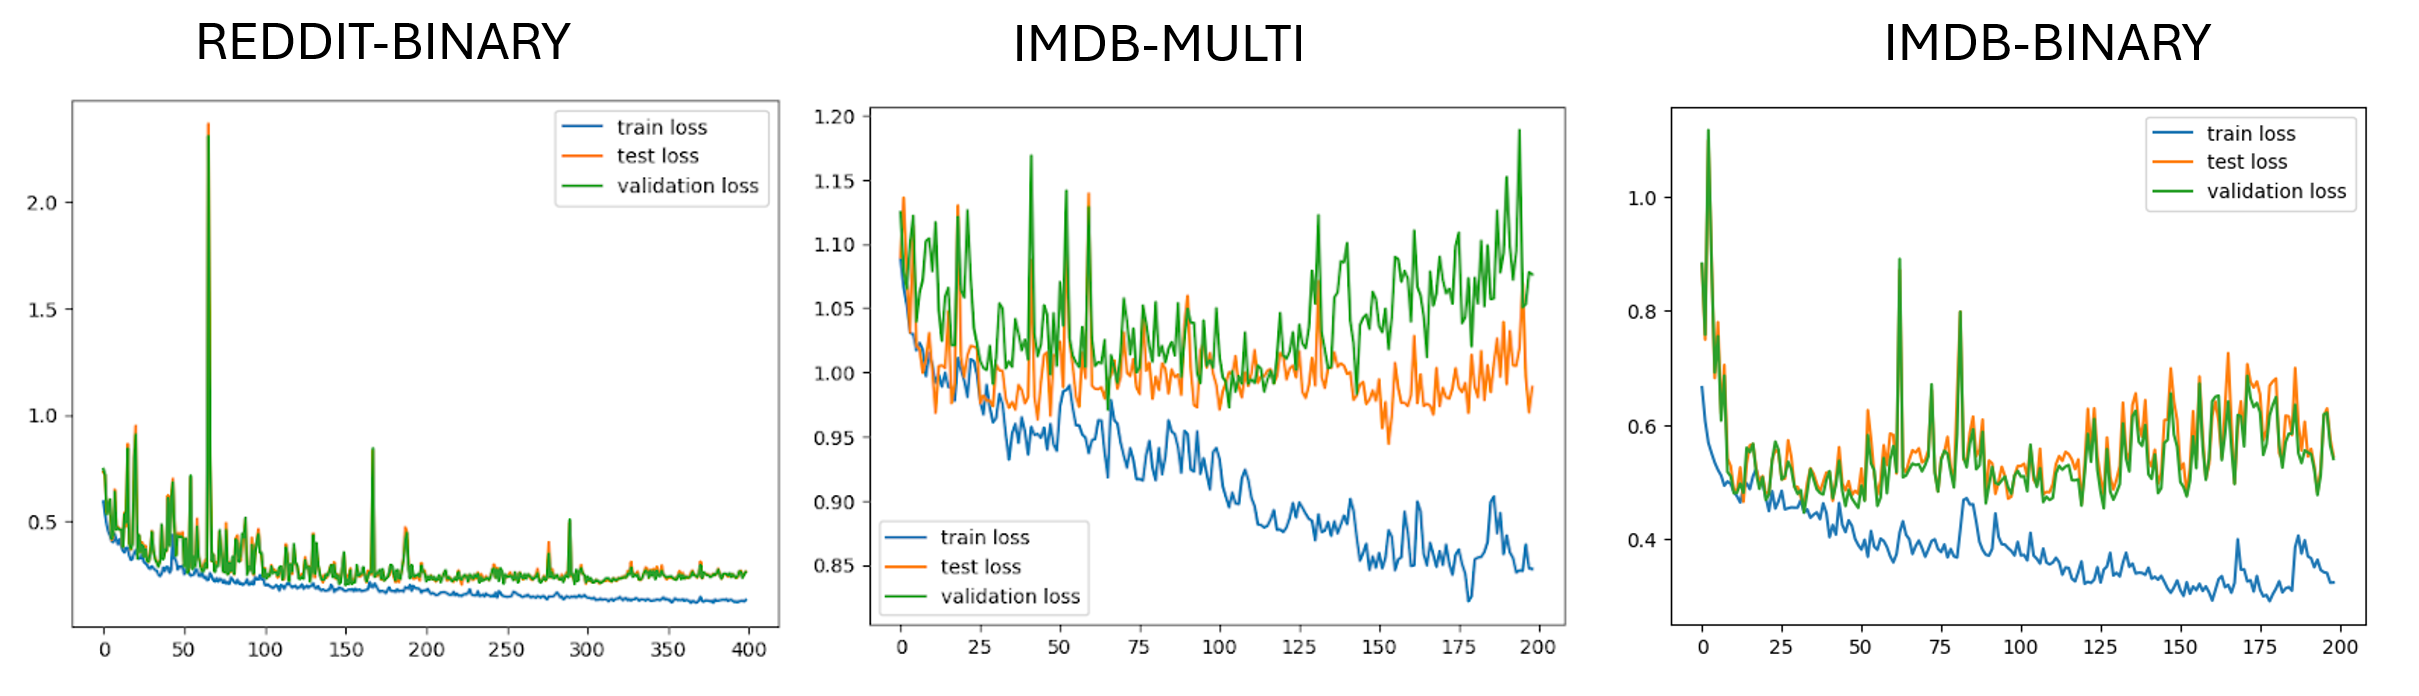
\includegraphics[width=\linewidth]{figures/AllLoss.PNG}
  \caption{The training/validation/test loss curves on IMDB-BINARY, IMDB-MULTI and REDDIT-BINARY with GIN as backbone.}
  \label{fig:Loss}
\end{figure*}

\begin{figure*}
  \centering
  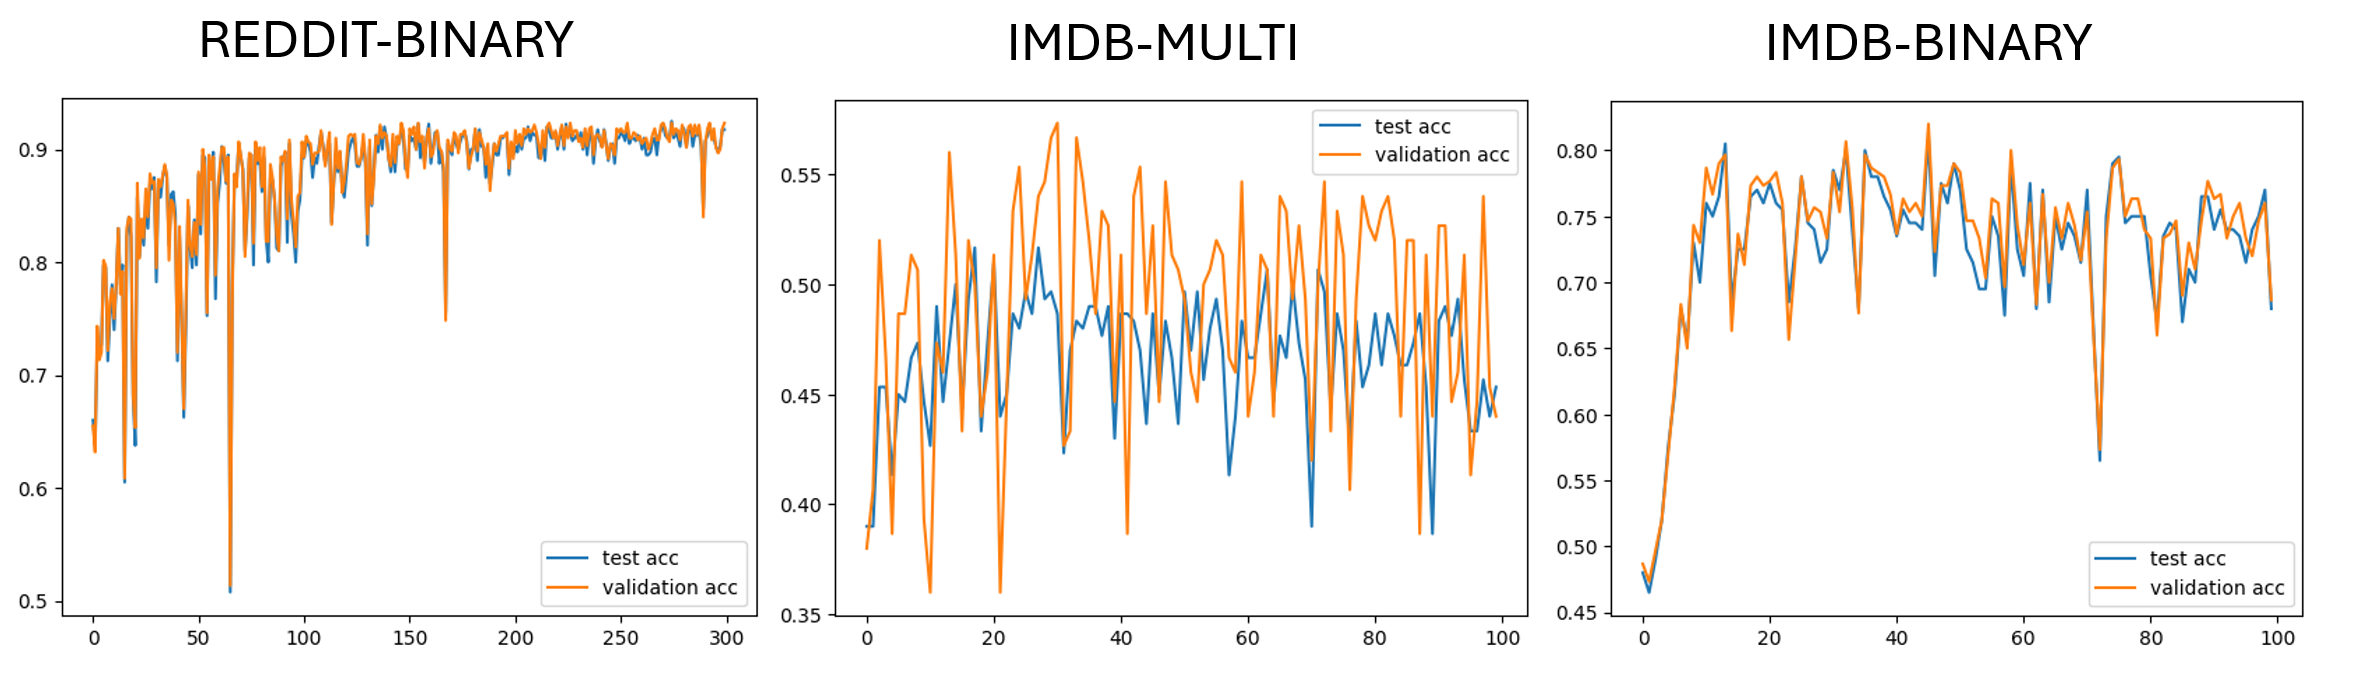
\includegraphics[width=\linewidth]{figures/AllAcc.PNG}
  \caption{The validation/test accuracy curves on IMDB-BINARY, IMDB-MULTI and REDDIT-BINARY with GIN as backbone before overfitting.}
  \label{fig:Acc}
\end{figure*}

\subsection{Tables}

The results we achieved are presented in Table \ref{results}. The reported results in \cite{han2022g} are based on 10 different runs. In our study, due to limited resources, each experiment was conducted only once. As indicated in Table \ref{results}, our results are consistent with those reported in \cite{han2022g}.

\begin{table*}[t] 
  \caption{Comparative Analysis of Our Findings with the Results from \cite{han2022g}.}
  \label{results}
  \begin{tabular}{cccc}
    \toprule
    Dataset & REDD-B & IMDB-B & IMDB-M \\
    \midrule
    G-Mixup \cite{han2022g} & $$92.90 \pm 0.87$$ & $$71.94 \pm 3.00$$ & $$50.46 \pm 1.49$$ \\
    Our G-Mixup  & 92.33 & 71.67 & 49.33\\
    \bottomrule
  \end{tabular}
\end{table*}


\subsection{Listings and Styles}

For the implementation we chose \texttt{Google Colab} for several reasons. First, the ability of \texttt{Google Colab} in handling compatible packages was a key factor. Another reason was related to the \texttt{torch\_geometric} package that, as mentioned before, is used to receive datasets presented in Table \ref{data}. This package requires \texttt{CUDA} to be installed on the system; however, it can be accessible with some commands on \texttt{Google Colab}. The last but not least reason is the provided \texttt{GPU} on \texttt{Google Colab} that can be helpful in speeding up the training process. The \texttt{Python} version used in our implementation is \texttt{3.10.12}.

Isomorphism, in the context of graph theory, is a concept used to determine if two graphs are essentially the same, differing only in the labeling of their vertices and the representation of their edges. In \cite{xu2018powerful} they designed a basic neural architecture, Graph Isomorphism Network (GIN), and demonstrated its discriminative and representational power. In this study, like the original paper \cite{han2022g}, we tested our method on GINs using \texttt{PyTorch}. Generally, in this implementation, \texttt{PyTorch} has been used for data processing and the training process.

All other details in the implementation, such as the division percentage of the training/testing/validation data, number of batches, and the number of hidden layers, are based on the original paper \cite{han2022g}.

Based on the reference paper \cite{han2022g}, the learning rate starts at 0:01 and decreases by 50\% after every 100 epochs. The batch size is set at 128. We divided the dataset into train, val, and test groups in a 7:1:2 ratio. 

\subsection{Math and Equations}

The mathematical part behind our implementation is exactly based on what is used in the \cite{han2022g}. These formula are as:

\begin{equation}
\text{Graphon Estimation:} \quad \mathcal{G} \rightarrow W_{\mathcal{G}}, \mathcal{H} \rightarrow W_{\mathcal{H}}
\end{equation}
\begin{equation}
\text{Graphon Mixup:} \quad W_{\mathcal{I}} = \lambda W_{\mathcal{G}} + (1 - \lambda) W_{\mathcal{H}}
\end{equation}
\begin{equation}
\text{Graph Generation:} \quad \{I_1, I_2, \ldots, I_m\} \sim \mathcal{G}(K, W_{\mathcal{I}})
\end{equation}
\begin{equation}
\text{Label Mixup:} \quad y_{\mathcal{I}} = \lambda y_{\mathcal{G}} + (1 - \lambda) y_{\mathcal{H}}
\end{equation}
where $W_{\mathcal{G}}$ and $W_{\mathcal{H}}$ are the graphon representations for the sets of graphs $\mathcal{G}$ and $\mathcal{H}$, respectively. The composite graphon is symbolized by $W_{\mathcal{I}}$, and the scalar $\lambda$ within the closed interval [0,1] serves as a balancing parameter to modulate the proportional contributions from each originating graph set. The assemblage of synthetic graphs derived from $W_{\mathcal{I}}$ is denoted as $\mathcal{I} = \{I_1, I_2, \dots, I_m\}$. The vectors $y_{\mathcal{G}} \in \mathbb{R}^C$ and $y_{\mathcal{H}} \in \mathbb{R}^C$ comprise the ground-truth labels for graphs in $\mathcal{G}$ and $\mathcal{H}$, respectively, where $C$ represents the count of classes. The labeling vector for synthetic graphs within the set $\mathcal{I}$ is represented as $y_{\mathcal{I}} \in \mathbb{R}^C$ \cite{han2022g}.


\section{Citations}

As mentioned in this article, the entire part of this study is based on \cite{han2022g}. In this report, we have endeavored to reference seminal studies in the domain of graph estimation and graph processing. There are additional pivotal studies employed in the original paper, such as \cite{lovasz2012large}, \cite{xu2021learning}, \cite{zhang2017mixup}, and \cite{zhang2020does}.


\begin{acks}
I would like to extend my gratitude to Professor Lingyang Chu, whose insightful guidance and unwavering support have been invaluable throughout the course of the project for the Machine Learning on Graphs course at McMaster University.
\end{acks}

%\clearpage

\bibliographystyle{ACM-Reference-Format}
\bibliography{sample}

\end{document}
\endinput
